% !TeX root = ../Avances.tex


\section{Conclusiones}

\begin{frame}{Conclusiones y trabajo a futuro}{Para una 12.5 nm AuNP parcialmente embebida entre un sustrato plano y una matriz}

  \begin{center}

  	\begin{tikzpicture}[node distance=1em and 1em,font=\small]

        \path (0,0) node [flowbox] (inc) {
        \fbtitle{Incrustación}\vphantom{yÖ}
	    \nodepart{two}
         \begin{minipage}{.28\textwidth}
         A lo más un octavo del  volumen en
         \begin{itemize}
			\item Sustrato $\to$ AuNP soportada
			\item Matriz $\to$ AuNP totalmente embebida
         \end{itemize}
         \end{minipage}
        };


	\node[flowbox,left=of inc] (trans) {
        \fbtitle{Transición}\vphantom{yÖ}
    \nodepart{two}
        \begin{minipage}{.28\textwidth}\begin{itemize}
			\item  Contribución mayormente dipolar.
  	\item Transición \textit{suave} entre los dos casos límites de Mie.
         \end{itemize}\end{minipage}
    };

    \node[flowbox,right=of inc] (pol) {
        \fbtitle{Iluminación}\vphantom{yÖ}
    \nodepart{two}
        \begin{minipage}{.28\textwidth}
        Resonancia y la distribución espacial del campo eléctrico
        \begin{itemize}
			\item  Pol. $s$:  no dependen de el ángulo de incidencia.
			\item Pol. $p$: sí dependen de el ángulo de incidencia.
         \end{itemize}
         $\theta_i \approx \theta_c$: Máximización de la extinción
		\end{minipage}
    };

    \node[below = of inc]{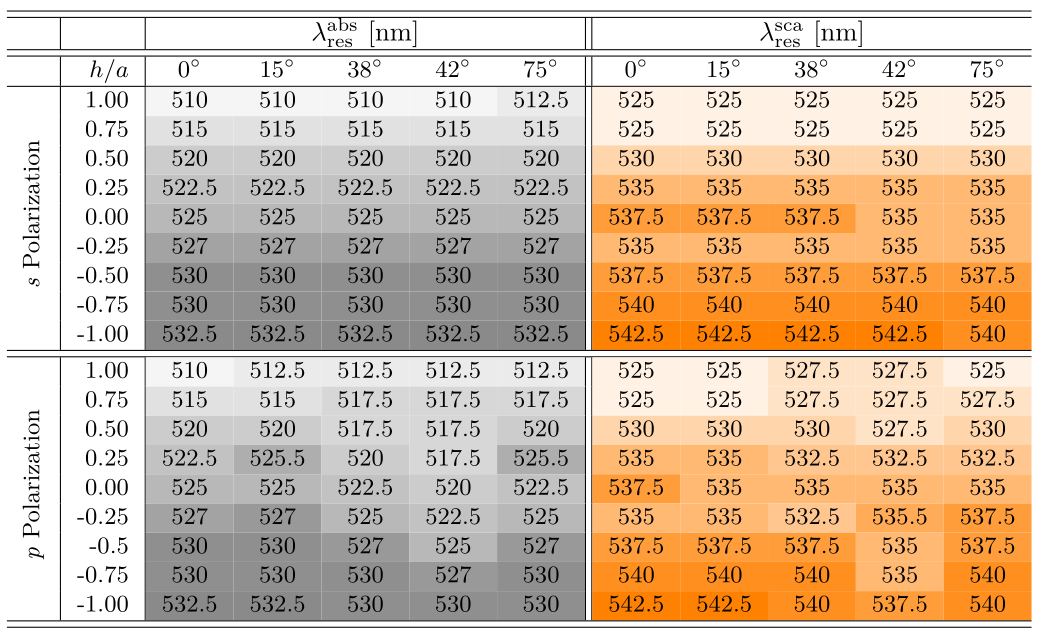
\includegraphics[scale  = .15]{Trans.png}};
    \node[below = of trans]{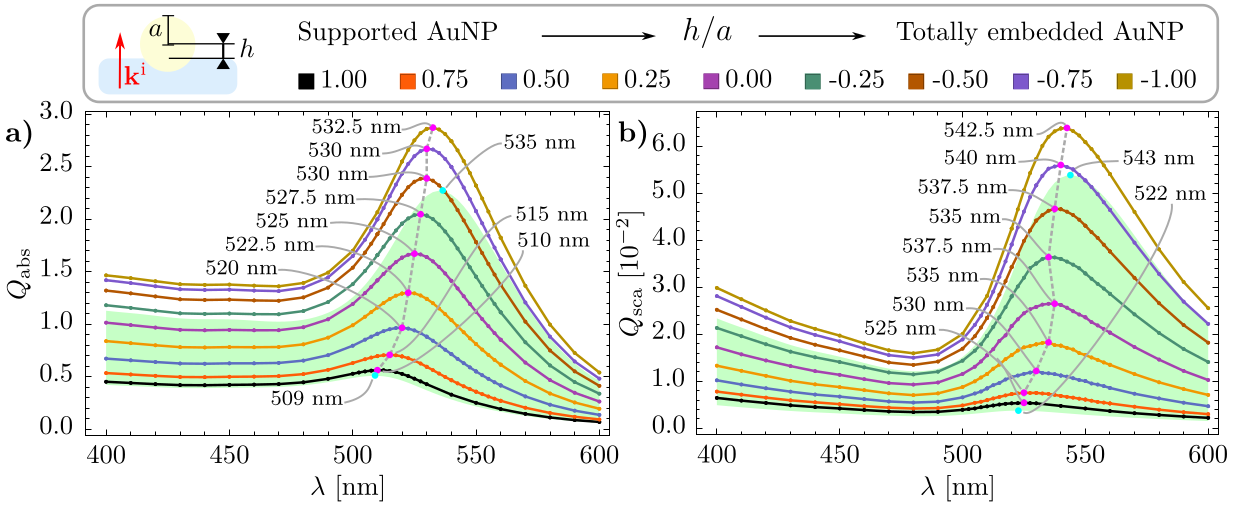
\includegraphics[scale  = .15]{Dip-Mie.png}};
    \node[below = of pol]{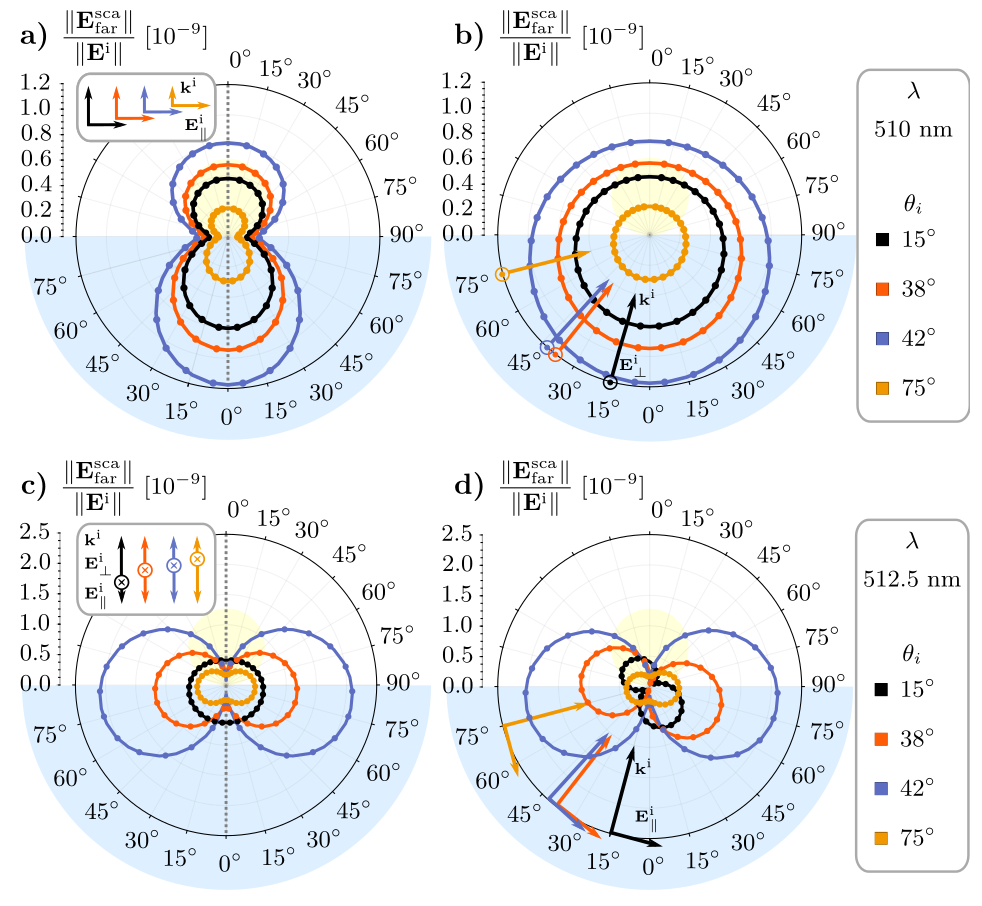
\includegraphics[scale  = .15]{Distribucion.png}};
%
 \path (-2.65,-5) node [flowbox]  (fut) {
        \fbtitle{Trabajo a futuro: Incrustación + Polarización}\vphantom{yÖ}
    \nodepart{two}
        \begin{minipage}{.6\textwidth}
         Metasuperficies de AuNP parcialmente incrustadas
        \begin{itemize}
  	\item Descripción de su respuesta óptica mediante teorías de medio efectivo
  	\item Metodología para medir su grado de incrustación promedio
         \end{itemize}
		\end{minipage}
    };


    \end{tikzpicture}
    \end{center}

\end{frame}



